\chapter{Formula Elaborations and Breakdowns}

This chapter provides detailed breakdowns of key mathematical formulas in the Elder Theory framework, addressing step-by-step analysis and visual explanations of complex expressions.

\section{Heliomorphic Transformation Formula Breakdown}

The heliomorphic transformation $T$ operates as:
\begin{equation}
T(\theta_1,\theta_2) = |\rho_1||\rho_2|e^{i(\phi_1 \oplus \phi_2)}
\end{equation}

\subsection{Step-by-Step Analysis}

This formula can be broken down into three fundamental components:

\textbf{Step 1: Magnitude Combination}
\begin{equation}
\text{Magnitude} = |\rho_1||\rho_2|
\end{equation}
The magnitudes $|\rho_1|$ and $|\rho_2|$ of the two heliomorphic parameters multiply directly. This represents the combination of the "strength" or "intensity" of the two knowledge representations.

\textbf{Step 2: Phase Composition Operation}
\begin{equation}
\text{Phase} = \phi_1 \oplus \phi_2
\end{equation}
The phases undergo a specialized composition operation $\oplus$, which is not simple addition but a heliomorphic phase composition that preserves the coupling structure between radial and angular components.

\textbf{Step 3: Complex Exponential Construction}
\begin{equation}
\text{Result} = \text{Magnitude} \times e^{i \times \text{Phase}}
\end{equation}
The final result combines the magnitude product with the exponential of the composed phase, maintaining the complex-valued structure essential for heliomorphic representations.

\section{Elder Field Representation Formula}

The Elder field representation $F$ is given by:
\begin{equation}
F_{\theta_E}(x) = \sum_{j=1}^{N} \gamma_j |x - r_j|^2 e^{i\phi_j} \hat{r}_j(x)
\end{equation}

\subsection{Visual Explanation of the Gamma Effect}

The parameter $\gamma_j$ controls multiple aspects of each field component:

\begin{figure}[h]
\centering
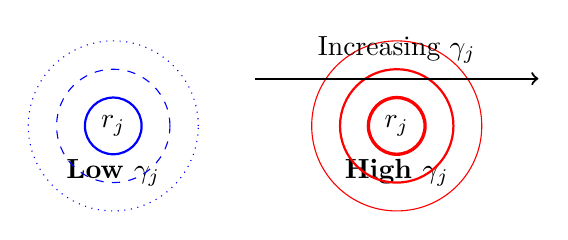
\begin{tikzpicture}[scale=1.2]
    % Field strength visualization
    \begin{scope}[shift={(0,0)}]
        \node at (0,-0.5) {\textbf{Low $\gamma_j$}};
        \draw[blue, thick] (0,0) circle (0.3);
        \draw[blue, dashed] (0,0) circle (0.6);
        \draw[blue, dotted] (0,0) circle (0.9);
        \node at (0,0) {$r_j$};
    \end{scope}
    
    \begin{scope}[shift={(3,0)}]
        \node at (0,-0.5) {\textbf{High $\gamma_j$}};
        \draw[red, very thick] (0,0) circle (0.3);
        \draw[red, thick] (0,0) circle (0.6);
        \draw[red] (0,0) circle (0.9);
        \node at (0,0) {$r_j$};
    \end{scope}
    
    % Effect arrows
    \draw[->, thick] (1.5, 0.5) to (4.5, 0.5);
    \node at (3, 0.8) {Increasing $\gamma_j$};
\end{tikzpicture}
\caption{Visual representation of how $\gamma_j$ affects field strength and influence radius around position $r_j$}
\end{figure}

\textbf{Effects of $\gamma_j$:}
\begin{itemize}
    \item \textbf{Field Strength}: Higher $\gamma_j$ increases the overall contribution of the $j$-th component
    \item \textbf{Influence Range}: The $|x - r_j|^2$ term creates a quadratic decay, but $\gamma_j$ scales this effect
    \item \textbf{Knowledge Concentration}: Large $\gamma_j$ values create "knowledge hotspots" where information is highly concentrated
    \item \textbf{System Balance}: The relative values of different $\gamma_j$ parameters determine the overall knowledge distribution across the Elder field
\end{itemize}

\section{Gravitational Field Parameters Introduction}

The Elder Theory framework operates within a continuous gravitational field where knowledge representations are governed by field strength parameters. This represents a fundamental shift from discrete parameter spaces to continuous field-theoretic descriptions.

\subsection{Gravitational Field Parameters (GFPs)}

Gravitational Field Parameters are continuous functions $\Gamma(x, t)$ that describe the local strength of the knowledge field at position $x$ and time $t$:

\begin{equation}
\Gamma(x, t) = \sum_{k} \alpha_k(t) G_k(x)
\end{equation}

where:
\begin{itemize}
    \item $G_k(x)$ are basis field functions (typically Gaussian or inverse-square)
    \item $\alpha_k(t)$ are time-dependent amplitudes
    \item The sum represents the superposition of multiple field sources
\end{itemize}

This gravitational field approach enables:
\begin{enumerate}
    \item \textbf{Continuous Knowledge Representation}: No discrete boundaries between knowledge domains
    \item \textbf{Dynamic Field Evolution}: Parameters can evolve smoothly over time
    \item \textbf{Natural Hierarchical Structure}: Field strength naturally decreases with distance from knowledge sources
    \item \textbf{Self-Organization}: System can autonomously organize through field interactions
\end{enumerate}

\section{Self-Organization Through Perturbation Response}

The Elder Heliosystem addresses orbital stability issues through an elegant self-organization mechanism based on perturbation response theory.

\subsection{Perturbation Response Framework}

When the system encounters destabilizing perturbations, it responds through three coordinated mechanisms:

\textbf{1. Adaptive Field Strength Adjustment}
\begin{equation}
\frac{d\Gamma}{dt} = -\alpha \nabla V_{\text{perturbation}} + \beta \mathcal{L}[\Gamma]
\end{equation}
where $\mathcal{L}$ is a stabilizing operator that counters destabilizing forces.

\textbf{2. Dynamic Orbital Correction}
\begin{equation}
\vec{F}_{\text{correction}} = -k_{\text{stab}} (\vec{r} - \vec{r}_{\text{equilibrium}})
\end{equation}
This provides a restoring force that guides entities back toward stable orbital configurations.

\textbf{3. Knowledge Transfer Rebalancing}
The system automatically adjusts knowledge transfer rates to maintain stability:
\begin{equation}
\tau_{\text{transfer}}^{\text{new}} = \tau_{\text{transfer}}^{\text{old}} \cdot \exp(-\lambda \cdot \text{instability\_measure})
\end{equation}

\subsection{Resolution of Stability Issues}

This perturbation response mechanism resolves the identified stability issues:

\begin{itemize}
    \item \textbf{Mentor Spiral Prevention}: Adaptive field strength prevents both inward collapse and outward escape
    \item \textbf{Erudite Stability}: Dynamic orbital correction maintains stable Erudite orbits around Mentors
    \item \textbf{Chaos Suppression}: Knowledge transfer rebalancing dampens chaotic dynamics
    \item \textbf{System Coherence}: The coordinated response maintains overall system integrity
\end{itemize}

The mathematical foundation ensures that perturbations drive the system toward greater stability rather than increased chaos, implementing a form of "learning from disturbance" that strengthens the overall framework.
